% Popular version of the mathematical-verification talk
% Compile: latexmk -pdf verification_talk_short.tex
\documentclass[aspectratio=169,11pt]{beamer}

\usetheme{default}
\usecolortheme{default}
\setbeamertemplate{navigation symbols}{}
\setbeamertemplate{itemize items}[circle]

\usepackage[T1]{fontenc}
\usepackage[utf8]{inputenc}
\usepackage{lmodern}
\usepackage{amsmath,amssymb}
\usepackage{booktabs}
\usepackage{graphicx}
\usepackage{xcolor}
\usepackage{array}

\definecolor{ink}{HTML}{12202C}
\definecolor{dtured}{HTML}{990000}
\definecolor{okgreen}{HTML}{2E7D32}
\definecolor{badred}{HTML}{B23A2E}
\definecolor{flagamber}{HTML}{9A7413}
\definecolor{slate}{HTML}{5A6B7A}
\definecolor{panel}{HTML}{F2F4F6}

\setbeamercolor{structure}{fg=dtured}
\setbeamercolor{normal text}{fg=ink}
\setbeamercolor{frametitle}{fg=ink}
\setbeamerfont{frametitle}{size=\large,series=\bfseries}
\setbeamercolor{block title}{bg=panel,fg=ink}
\setbeamercolor{block body}{bg=panel!60,fg=ink}
\setbeamercolor{alerted text}{fg=dtured}

\setbeamertemplate{frametitle}{%
  \vspace{0.35cm}%
  \insertframetitle\par
  \vspace{-0.15cm}{\color{dtured}\rule{\textwidth}{1pt}}}
\setbeamertemplate{footline}{%
  \hfill{\color{slate}\scriptsize\insertframenumber}\hspace{0.4cm}\vspace{0.2cm}}

\newcommand{\code}[1]{{\ttfamily\small #1}}
\newcommand{\PASS}{{\color{okgreen}\bfseries PASS}}
\newcommand{\FAIL}{{\color{badred}\bfseries FAIL}}
\newcommand{\FLAG}{{\color{flagamber}\bfseries FLAG}}
\newcommand{\NC}{{\color{slate}\bfseries NOT CHECKED}}

\title{\bfseries Can we run the mathematics\\in a research paper?}
\subtitle{A practical audit of equations and reported results}
\author{Jeppe Rich}
\institute{DTU Management}
\date{\today}

\begin{document}

\begin{frame}[plain]
  \titlepage
\end{frame}

\begin{frame}{Some errors survive every careful reading}
  \begin{enumerate}\itemsep0.8em
    \item A term disappears during a long derivation.
    \item A calibration no longer reproduces its own table.
    \item An optimizer is asked to solve a different problem from the one described.
  \end{enumerate}
  \vfill
  \begin{block}{}
    \centering
    These errors look plausible on the page. They become obvious when the claim is executed.
  \end{block}
\end{frame}

\begin{frame}{Producing a result is hard; checking it is often cheap}
  \begin{center}
  \begin{tabular}{@{}p{0.42\textwidth}p{0.23\textwidth}p{0.25\textwidth}@{}}
    \toprule
    \textbf{Claim} & \textbf{Produce} & \textbf{Check} \\
    \midrule
    Algebraic identity & derive it & simplify left $-$ right \\[0.35em]
    Calibrated number & estimate it & substitute and compare \\[0.35em]
    Feasible solution & search for it & recompute constraints \\[0.35em]
    Claimed optimum & solve a hard problem & compare value and bound \\
    \bottomrule
  \end{tabular}
  \end{center}
  \vfill
  \centering\large\alert{Verification exploits the gap between the last two columns.}
\end{frame}

\begin{frame}{The paper becomes an executable checklist}
  \begin{columns}[T]
    \begin{column}{0.46\textwidth}
      \begin{block}{1. Translate}
        Turn each equation, implication, table entry, and solver claim into a small executable check.
      \end{block}
    \end{column}
    \begin{column}{0.46\textwidth}
      \begin{block}{2. Judge}
        The computer returns \PASS, \FAIL, or \NC. It does not decide whether an argument sounds convincing.
      \end{block}
    \end{column}
  \end{columns}
  \vfill
  \begin{block}{The rule}
    \centering
    Every mathematical claim is either executed or explicitly listed as not executed.
  \end{block}
\end{frame}

\begin{frame}{A human translates; the machine checks}
  \begin{center}
    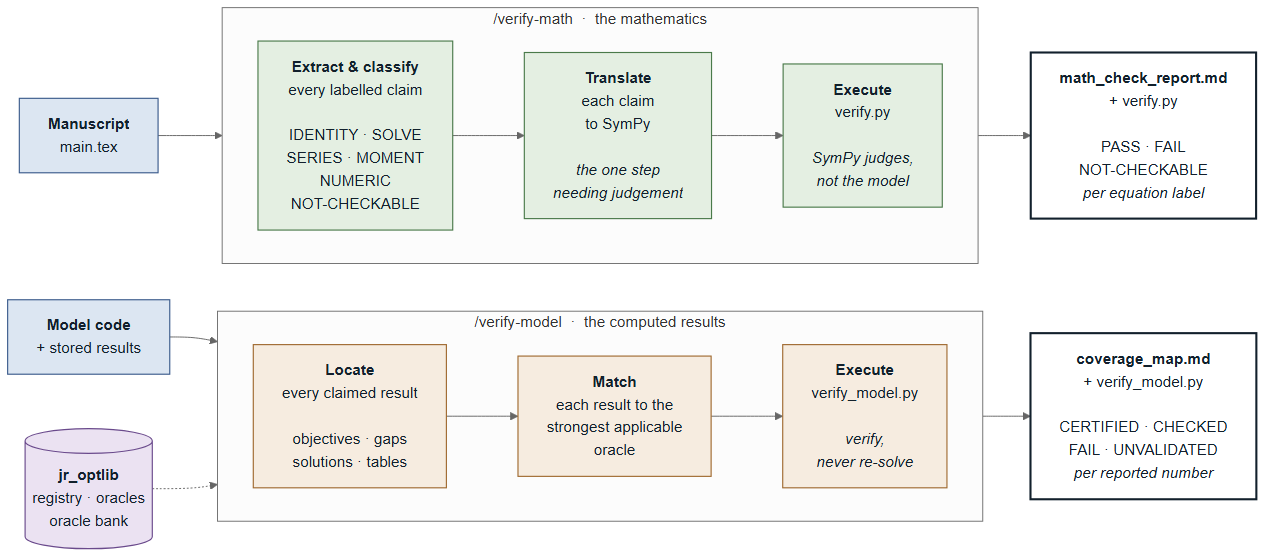
\includegraphics[width=0.82\textwidth]{workflow.png}
  \end{center}
  \vfill
  \centering\small
  The report shows the original claim, the executable version, the verdict, and the boundary of coverage.
\end{frame}

\begin{frame}{Inside the optimization library}
  \begin{center}
  \begin{tabular}{c@{\quad$\longrightarrow$\quad}c@{\quad$\longrightarrow$\quad}c}
    \fcolorbox{dtured}{panel}{\parbox{0.21\textwidth}{\centering\textbf{Paper model}\\data, assumptions, claim}}
    &
    \fcolorbox{dtured}{panel}{\parbox{0.24\textwidth}{\centering\textbf{Vetted primitive}\\IPF, transport, MIP, DP, sampling}}
    &
    \fcolorbox{dtured}{panel}{\parbox{0.22\textwidth}{\centering\textbf{Candidate result}\\solution, value, bound}}
  \end{tabular}
  \end{center}
  \vspace{0.8em}
  \begin{center}
    $\Downarrow$ \hspace{0.43\textwidth} $\Downarrow$
  \end{center}
  \vspace{-0.4em}
  \begin{columns}[T]
    \begin{column}{0.47\textwidth}
      \begin{block}{Solver backend: produce}
        NumPy/SciPy, OR-Tools, PuLP, or a custom algorithm. \textbf{Gurobi is optional}: used for selected MIPs, MIQPs, and exact benchmark bounds.
      \end{block}
    \end{column}
    \begin{column}{0.47\textwidth}
      \begin{block}{Independent oracle: judge}
        Recompute feasibility and value; compare a dual bound, exact solver, brute-force instance, reference implementation, or invariant.
      \end{block}
    \end{column}
  \end{columns}
  \vfill
  \centering\small
  The harness converts the oracle outputs into \textbf{CERTIFIED / CHECKED / FAIL / UNVALIDATED}. At submission, the paper pins the library commit.
\end{frame}

\begin{frame}{First test: one of our own papers}
  \begin{columns}[T]
    \begin{column}{0.40\textwidth}
      \centering
      {\fontsize{34}{38}\selectfont\bfseries 58}\par
      executable checks
    \end{column}
    \begin{column}{0.54\textwidth}
      \begin{itemize}\itemsep0.7em
        \item 55 passed immediately.
        \item Three calibrated percentages failed.
        \item All three failures traced to one stale calibration.
        \item Correcting one input restored all three results.
      \end{itemize}
    \end{column}
  \end{columns}
  \vfill
  \begin{block}{}
    The equations were not difficult. The problem was that nobody had substituted the final parameters back into them.
  \end{block}
\end{frame}

\begin{frame}{Then we took three papers at random}
  \begin{itemize}\itemsep0.7em
    \item Three newly published papers were supplied without screening.
    \item All appeared in leading transportation journals.
    \item We checked the papers as printed, not the authors or their reputations.
    \item Names are withheld: the point is the failure mode, not attribution.
  \end{itemize}
  \vfill
  \begin{block}{Important boundary}
    These are internal-consistency findings. Unavailable source code could silently correct a printed formulation.
  \end{block}
\end{frame}

\begin{frame}{Anonymous paper A: the objective changes direction}
  The text asks the model to
  \[
    \text{minimize pollution}\qquad\text{and}\qquad\alert{\text{maximize parking flow}}.
  \]
  But the printed optimization problem is
  \[
    \min\;\bigl(J_{\mathrm{pollution}},J_{\mathrm{parking}}\bigr),
  \]
  and the weighted solver gives both quantities positive weights.
  \vfill
  \begin{block}{What goes wrong}
    The optimizer is rewarded for reducing parking flow---the opposite of the stated policy objective. The reported table confirms that parking flow is stored as a positive quantity, not as a loss.
  \end{block}
\end{frame}

\begin{frame}{Anonymous paper B: variance is used as a scale}
  The method says that the scaling matrix contains \textbf{standard deviations}. The example states a variance of $4$, but inserts $4$ rather than $\sqrt{4}=2$.
  \vfill
  \begin{center}
  \begin{tabular}{@{}lcc@{}}
    \toprule
     & \textbf{Scale used} & \textbf{Reported metric} \\
    \midrule
    Printed example & $4$ & $11.52$ \\
    Consistent with variance $4$ & $2$ & $12.50$ \\
    \bottomrule
  \end{tabular}
  \end{center}
  \vfill
  The same paper's convergence proof first derives $r^*\ge r$ and then concludes $r^*<r$ from the same premise.
  \vfill
  {\color{slate}\small Arithmetic independently recomputed; the algorithm may still be correct despite the broken printed proof.}
\end{frame}

\begin{frame}{Anonymous paper C: objective and algorithm diverge}
  The stated objective is an undiscounted sum:
  \[
    \mathbb{E}\!\left[\sum_{t=0}^{T} r_t\right].
  \]
  The Bellman equation and experiments instead discount the future:
  \[
    V(s_t)=\max_a\mathbb{E}\!\left[r_t+\alert{0.9}\,V(s_{t+1})\right].
  \]
  \vfill
  \begin{block}{A second formulation gap}
    A relocation-time constraint applies to every possible destination, even when that destination is not selected. It is missing the condition ``if this relocation is chosen.''
  \end{block}
\end{frame}

\begin{frame}{Four papers: what passed, and what was flagged}
  \begin{center}
  \small
  \begin{tabular}{@{}p{0.16\textwidth}p{0.31\textwidth}p{0.39\textwidth}@{}}
    \toprule
    \textbf{Paper} & \textbf{Correct checks observed} & \textbf{Flags} \\
    \midrule
    Anonymous A & 5/5 numerical spot checks & 1 objective-direction inconsistency \\[0.45em]
    Anonymous B & Printed arithmetic reproduced & 1 variance/scale inconsistency; 1 contradictory proof step \\[0.45em]
    Anonymous C & 2/2 accounting identities & 2 formulation gaps: discounting and relocation condition \\[0.45em]
    Famous benchmark & 49/49 derivations & 1 unstated side condition; 3 strictness gaps \\
    \bottomrule
  \end{tabular}
  \end{center}
  \vfill
  {\color{slate}\scriptsize The famous-paper row is a complete derivation audit. The anonymous rows are targeted internal-consistency screens, so their counts are not coverage totals.}
\end{frame}

\begin{frame}{A famous stress test: prospect theory}
  We also transcribed every stated derivation in a landmark economics paper and ran them end to end.
  \vfill
  \begin{center}
  \begin{tabular}{@{}lr@{}}
    \toprule
    Checks run & \textbf{49} \\
    Passed & \textbf{49} \\
    Failed & 0 \\
    Unstated side condition found & \textbf{1} \\
    Strictness gaps & 3 \\
    \bottomrule
  \end{tabular}
  \end{center}
  \vfill
  The result is not ``machines find mistakes everywhere.'' It is that they distinguish sound derivations from the few steps that need an extra condition.
\end{frame}

\begin{frame}{What this does---and does not---establish}
  \begin{columns}[T]
    \begin{column}{0.46\textwidth}
      \begin{block}{It can establish}
        \begin{itemize}
          \item identities and implications;
          \item numerical consistency;
          \item feasibility and objective values;
          \item explicit coverage and omissions.
        \end{itemize}
      \end{block}
    \end{column}
    \begin{column}{0.46\textwidth}
      \begin{block}{It cannot establish}
        \begin{itemize}
          \item that the translation is faithful;
          \item that assumptions are realistic;
          \item generality from a few examples;
          \item a formal proof of the whole paper.
        \end{itemize}
      \end{block}
    \end{column}
  \end{columns}
  \vfill
  \centering\alert{This is an audit of stated mathematics, not formal verification.}
\end{frame}

\begin{frame}{Why the modest version matters}
  \begin{itemize}\itemsep0.9em
    \item Formal proof systems offer stronger guarantees, but require specialist effort.
    \item This approach works with the paper researchers already write.
    \item Failures point to a specific equation, table entry, or assumption.
    \item The cost is low enough to run before every submission.
  \end{itemize}
  \vfill
  \begin{block}{}
    \centering\large
    A limited check that runs on every paper can prevent more errors than a perfect check that is never attempted.
  \end{block}
\end{frame}

\begin{frame}{Do not merely proofread the mathematics}
  \vfill
  \begin{center}
    {\fontsize{30}{36}\selectfont\bfseries Execute it.}
  \end{center}
  \vfill
  \begin{enumerate}\itemsep0.6em
    \item Turn every checkable claim into an executable statement.
    \item Let the machine judge equality, feasibility, and arithmetic.
    \item Report both what passed and what was never checked.
  \end{enumerate}
  \vfill
  \centering
  \alert{The goal is not perfect certainty. It is fewer avoidable errors.}
\end{frame}

\end{document}
